\documentclass[11pt]{article}

\usepackage[a4paper,margin=2.4cm]{geometry}
\usepackage{amsmath,amssymb}
\usepackage{booktabs}
\usepackage{graphicx}
\usepackage{multirow}
\usepackage[round,authoryear]{natbib}
\usepackage[hidelinks]{hyperref}
\usepackage{microtype}
\usepackage{url}

\graphicspath{{./}}
\renewcommand{\tablename}{Supplementary Table}
\renewcommand{\figurename}{Supplementary Figure}

\title{\textbf{Supplementary Information}\\[0.5em]
Evaluation Choices Determine Apparent Quantum-Kernel Robustness under Distribution Shift}
\author{Roberto Fern\'andez-Barrios, Iker Pastor-L\'opez,\\
Asier Gonz\'alez-Santocildes, and Pablo Garc\'ia Bringas\\[0.4em]
\small Faculty of Engineering, University of Deusto, Bilbao, Spain}
\date{}

\begin{document}
\maketitle

\section*{Supplementary Note: Scope}

This document provides the construction details, complete candidate definitions, secondary analyses, and reporting specifications that support the main article. The primary estimand and conclusions are unchanged: the eight scenario-groups are fixed case studies; the headline comparison selects configurations without out-of-distribution (OOD) labels, tunes regularization from training data only, and gives the two extended kernel families equal candidate budgets. All tables and figures are generated from the frozen machine-readable analysis artifact.

\section*{Supplementary Note: Dataset and shift construction}
\label{supp:data}

\subsection*{Common split structure}

We study binary malware or network-attack classification using EMBER \citep{anderson2018ember}, UNSW-NB15 \citep{moustafa2015unsw}, and ToN-IoT \citep{alsaedi2020toniot}. Every setting has a training set $T$, an in-distribution test set $S_{\mathrm{ID}}$, and a shifted test set $S_{\mathrm{OOD}}$. Classical and quantum kernels always use the same samples. Class balance is preserved in the constructed splits, so the measured change is not driven by a prevalence shift.

\subsection*{EMBER label-conditional tail shifts}

The EMBER analysis uses the histogram and byte-entropy feature blocks and two reproducible stress tests. Both select OOD samples within each class. They are therefore described as \emph{label-conditional tail shifts}, not as certified covariate shifts: conditioning the split on the class does not establish that $P(Y\mid X)$ is invariant.

In the $m1$ construction, each sample receives a sparsity score equal to the number of non-zero entries in the selected feature block. The OOD set contains the low- and high-score extremes within each class. The remaining samples form an ID pool from which training and ID test sets are sampled stratifiably.

In the $m2$ construction, the final training set is fixed first. Class-conditional centroids are computed in a MaxAbs-scaled, TruncatedSVD space fitted on training data only. Every non-training sample is scored by its Euclidean distance to its own-class centroid. The low- and high-distance extremes within each class form the exact-size OOD set, and the ID test set is drawn from the remainder. This construction therefore probes unusual geometry relative to the final training set.

\subsection*{Network-flow scenarios}

The network experiments define UNSW-NB15 DoS, UNSW-NB15 Reconnaissance, and ToN-IoT Scanning scenarios. Numeric-only preparation removes identifiers, label-derived columns, and categorical protocol fields, retaining 39 UNSW-NB15 features and 89 ToN-IoT features. The largest observed absolute feature-label correlation is $0.62$, attained by a legitimate traffic feature rather than a label-derived field; the public artifact includes the leakage audit.

Each scenario has a reference pool and a current pool. Two mechanisms are applied. The \emph{m2-centroid} mechanism is the network analogue of EMBER $m2$: class-conditional centroids are fitted in a train-only MaxAbs+TruncatedSVD space and within-class distance tails define the OOD pool. The \emph{attack-campaign regime shift} uses no geometric selection. Training and ID samples come from benign traffic plus all non-target attack categories, whereas OOD samples come from benign traffic plus the held-out target campaign. For UNSW-NB15, the pools also use different official capture partitions. This is consequently an unseen-campaign plus capture-partition shift, not a timestamp-defined temporal split.

\section*{Supplementary Note: Controlled kernel-swap protocol}
\label{supp:protocol}

\subsection*{Preprocessing and classifiers}

All models use MaxAbs scaling followed by TruncatedSVD with
\[
d\in\{4,6,8,10,12\}.
\]
For fidelity kernels, each reduced coordinate is mapped linearly to $[0,\pi]$ before the angle-scale factor is applied. Preprocessing is fitted using the training split and shared across families.

Two learners consume precomputed Gram matrices. The primary learner is support-vector classification (SVC). The secondary learner is binary Gaussian-process classification using the standard Laplace approximation with a logistic link \citep{rasmussen2006gpml}. The GP classifier supplies approximate probabilities for the uncertainty analysis; no post-hoc calibration is applied. Comparisons are always made within a classifier.

\subsection*{Kernel candidates}

The customary classical reference contains a cosine-normalized linear kernel and the radial-basis-function (RBF) kernel
\[
K_{\mathrm{RBF}}(x,x')=\exp[-\gamma\|x-x'\|_2^2].
\]
The extended classical family adds cosine-normalized polynomial kernels of degrees 2 and 3, the Laplacian kernel, and Mat\'ern kernels with $\nu\in\{3/2,5/2\}$. Base length scales are set by the median pairwise training distance. RBF, Laplacian, and Mat\'ern candidates sweep factors
\[
f\in\{0.1,0.3,1,3,10\}
\]
relative to their base scale.

The quantum family uses fidelity kernels
\[
K_Q(x,x')=\left|\langle\phi_Q(x)\mid\phi_Q(x')\rangle\right|^2
\]
from four commonly used feature-map configurations: ZZ maps with one and two repetitions, a PauliXZ map with one repetition, and a Z map. Each is evaluated at angle scales $\{0.5,1,2\}$. These candidates cover representative low-qubit fidelity constructions rather than the full quantum-kernel design space.

\subsection*{Regularization, deployment selection, and candidate budgets}

For each of the 23 classical and 12 quantum kernel geometries, SVC regularization is selected from
\[
C\in\{0.01,0.1,1,10,100\}
\]
by five-fold stratified cross-validation on the training Gram matrix. Ties are broken toward the smaller $C$. Because $C$ is resolved within each configuration before the family comparison, it is not counted as another family-level candidate.

The primary P1$'$ deployment protocol divides the original ID test split deterministically and class-stratifiably into an ID-validation half and a disjoint ID-test half. Within a run and family, the configuration with the highest ID-validation balanced accuracy is deployed and evaluated on the untouched ID-test and OOD-test splits. No OOD label enters selection.

The quantum pool contains 60 candidates in full-coverage groups and 20 in reduced-coverage groups after combining feature map, angle scale, and dimension. The frozen primary analysis compares it with an equal-size sample from the extended classical pool. Five thousand subsamples and three sampling schemes characterize budget sensitivity. The full 115-candidate classical pool is retained as a secondary sensitivity. P2 uses OOD information from other realizations and P3 selects on the same OOD test labels; neither is a deployable primary analysis.

\subsection*{Repeated runs and fixed-case inference}

Each setting is realized with five split seeds and three model seeds, giving fifteen pipeline realizations per evaluated configuration. The eight scenario-groups share source pools and are not exchangeable; in particular, some constructed EMBER OOD samples recur across master seeds. The analysis therefore treats scenario-groups as fixed case studies. Per-group quantum-minus-classical effects are means over the five split-seed clusters with conditional $t$ intervals. BCa bootstrap and leave-one-split-out calculations are secondary diagnostics. Across groups, we report dataset-equal means and leave-one-dataset-out ranges, not a population $p$-value.

\begin{table}[t]
\centering
\caption{Complete experimental protocol.}
\label{supp:tab_protocol}
\small
\setlength{\tabcolsep}{4pt}
\begin{tabular}{lp{10.5cm}}
\toprule
Component & Specification \\
\midrule
Scenarios & EMBER; UNSW-NB15 DoS; UNSW-NB15 Reconnaissance; ToN-IoT Scanning \\
Shift mechanisms & EMBER $m1$ and $m2$; network m2-centroid and held-out attack-campaign shift \\
Master seeds & 42, 123, 999 \\
Split seeds & 42, 123, 999, 7, 2024 \\
Model seeds & 42, 123, 999 \\
Runs & $5\times3=15$ per evaluated configuration \\
Sizes $(n_{\mathrm{train}},n_{\mathrm{ID}},n_{\mathrm{OOD}})$ & $(1000,500,500)$, $(2000,1000,1000)$, $(4000,1800,1800)$ \\
Dimensions & $d\in\{4,6,8,10,12\}$ \\
Classifiers & Precomputed-kernel SVC; precomputed-kernel Laplace GP classifier \\
Classical family & Linear, RBF, polynomial (2, 3), Laplacian, Mat\'ern ($3/2$, $5/2$) \\
Quantum family & ZZ (1 and 2 repetitions), PauliXZ, Z map; fidelity overlap \\
Scale freedom & Five classical length-scale factors; three quantum angle factors \\
Regularization & Per-configuration SVC $C$, five-fold training-only cross-validation \\
Primary selection & P1$'$ ID-validation; no OOD labels; equal candidate budgets \\
Inference & Fixed-case conditional intervals; dataset-equal summaries; no population $p$-value \\
\bottomrule
\end{tabular}
\end{table}

\section*{Supplementary Note: Metrics and geometry descriptors}
\label{supp:metrics}

Balanced accuracy on $S_{\mathrm{OOD}}$ is the primary endpoint. Family effects are
\[
\Delta_{\mathrm{OOD}}=
\mathrm{BAcc}^{(Q)}_{\mathrm{OOD}}-
\mathrm{BAcc}^{(C)}_{\mathrm{OOD}},
\]
with positive values favouring the quantum family. ID balanced accuracy and the ID-to-OOD drop are secondary. The GP analysis additionally records log loss, Brier score, expected calibration error with 15 equal-width bins \citep{guo2017calibration}, and predictive entropy.

For a positive-semidefinite training Gram matrix with eigenvalues $\lambda_i$ and $p_i=\lambda_i/\sum_j\lambda_j$, effective rank is
\[
r_{\mathrm{eff}}=\exp\left(-\sum_i p_i\log p_i\right)
\]
\citep{roy2007effective}. Centered kernel-target alignment (KTA) for labels $y\in\{-1,+1\}^n$ is
\[
\mathrm{KTA}(K,y)=
\frac{\langle K_c,yy^\top\rangle_F}
{n\|K_c\|_F},
\]
where $K_c$ is doubly centered \citep{cristianini2001kta,cortes2012centeredalignment}. KTA is computed separately on training, ID, and OOD blocks.

We also record the mean and standard deviation of off-diagonal entries, cross-split similarities, and the geometric difference
\[
g(K_C\!\rightarrow\!K_Q)=
\left\|
\sqrt{K_Q}(K_C+\lambda n I)^{-1}\sqrt{K_Q}
\right\|_\infty^{1/2}
\]
\citep{huang2021powerofdata}. Geometry-performance association is assessed within scenario-groups across all kernel-dimension cells using Spearman correlation, with partial association controlling for family and length scale. Leave-one-dataset-out prediction tests portability, and nearest-effective-rank matching compares families within run and dimension. These are observational diagnostics, not causal estimates or deployable selectors.

\section*{Supplementary Note: Why the oracle comparison is optimistic}
\label{supp:oracle}

The initial evaluation selected the best candidate using the OOD test labels themselves and left SVC regularization at $C=1$. Against linear and RBF kernels, this produces a mean EMBER OOD effect of $+0.0374$ for SVC and $+0.0283$ for the GP classifier (Table~\ref{supp:tab_oracle}). Expanding the classical family nearly removes this apparent gain even before honest selection is imposed. Because the same target labels select and score the candidate, these values are descriptive upper bounds rather than deployable effect estimates.

\begin{table}[t]
\centering
\caption{Descriptive EMBER oracle results under fixed $C=1$ (18 correlated settings). Mean and median effects are quantum minus classical balanced accuracy.}
\label{supp:tab_oracle}
\small
\begin{tabular}{llcccc}
\toprule
Selection & Classifier & Classical reference & Q wins & Mean $\Delta$ & Median $\Delta$ \\
\midrule
\multirow{4}{*}{Best-by-OOD}
 & SVC & linear+RBF & 17/18 & $+0.0374$ & $+0.0426$ \\
 & SVC & extended & 15/18 & $+0.0044$ & $+0.0064$ \\
 & GP & linear+RBF & 15/18 & $+0.0283$ & $+0.0339$ \\
 & GP & extended & 11/18 & $+0.0023$ & $+0.0029$ \\
\midrule
\multirow{4}{*}{Best-by-ID}
 & SVC & linear+RBF & 18/18 & $+0.0775$ & $+0.0794$ \\
 & SVC & extended & 18/18 & $+0.0149$ & $+0.0152$ \\
 & GP & linear+RBF & 18/18 & $+0.0649$ & $+0.0664$ \\
 & GP & extended & 18/18 & $+0.0192$ & $+0.0166$ \\
\bottomrule
\end{tabular}
\end{table}

\section*{Supplementary Note: Per-group geometry and rank matching}
\label{supp:geometry}

Table~\ref{supp:tab_geometry} supplies the values summarized graphically in the main article. Effective-rank association changes sign across regimes, whereas OOD KTA is more consistently positive. Nearest-rank matching favours the classical member in median accuracy in every group.

\begin{table}[t]
\centering
\caption{Geometry-OOD association and nearest-effective-rank matching for SVC. ``Partial'' controls for kernel family and length scale.}
\label{supp:tab_geometry}
\small
\setlength{\tabcolsep}{4pt}
\begin{tabular}{lccccc}
\toprule
Scenario & $\rho$ rank & Partial & $\rho$ KTA & Matched $\Delta$ & Q better \\
\midrule
EMBER $m1$ & $+0.32$ & $+0.36$ & $+0.30$ & $-0.0094$ & 33\% \\
EMBER $m2$ & $+0.80$ & $+0.82$ & $+0.63$ & $-0.0089$ & 22\% \\
UNSW-DoS (campaign) & $+0.44$ & $+0.41$ & $+0.64$ & $-0.0089$ & 27\% \\
UNSW-DoS (constructed) & $-0.14$ & $-0.08$ & $+0.39$ & $-0.0057$ & 29\% \\
UNSW-Recon (campaign) & $+0.06$ & $+0.06$ & $+0.22$ & $-0.0047$ & 37\% \\
UNSW-Recon (constructed) & $-0.15$ & $-0.08$ & $+0.37$ & $-0.0061$ & 30\% \\
ToN-IoT (campaign) & $+0.25$ & $+0.27$ & $+0.46$ & $-0.0060$ & 24\% \\
ToN-IoT (constructed) & $+0.65$ & $+0.63$ & $+0.59$ & $-0.0013$ & 35\% \\
\bottomrule
\end{tabular}
\end{table}

\section*{Supplementary Note: Predictive uncertainty under shift}
\label{supp:uncertainty}

The Laplace GP probabilities are approximate and are assessed rather than assumed to be calibrated. Predictive entropy rises from ID to OOD for both families in every scenario-group. Expected calibration error changes moderately and comparably (Figure~\ref{supp:fig_uncertainty}). Because the honestly selected fidelity kernels have no accuracy advantage, the uncertainty analysis provides no evidence of a calibration benefit unavailable to the classical family. Entropy increase alone is not evidence of good calibration.

\begin{figure}[t]
\centering
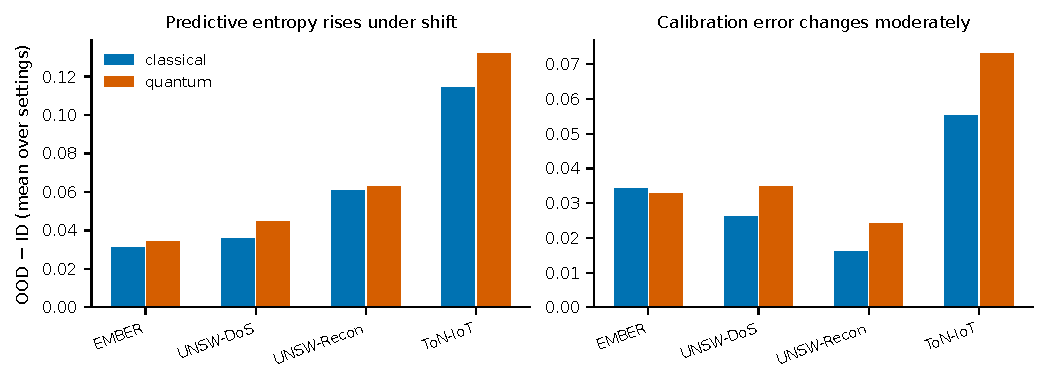
\includegraphics[width=\textwidth]{fig_v4_uncertainty.pdf}
\caption{Mean ID-to-OOD change in predictive entropy (left) and expected calibration error (right) for the P1$'$-selected configuration of each family, aggregated by dataset.}
\label{supp:fig_uncertainty}
\end{figure}

\section*{Supplementary Note: Finite-shot fidelity-estimation model}
\label{supp:shots}

For $s\in\{128,512,2048,8192\}$ shots, every exact fidelity $p$ is replaced by a binomial estimate $\hat p\sim\mathrm{Binomial}(s,p)/s$. Square training blocks are symmetrized, clipped to $[0,1]$, assigned an exact unit diagonal, and projected to the positive-semidefinite cone. Rectangular test blocks receive sampling and clipping only. The procedure isolates fidelity-estimation noise; it does not model a specific device, circuit compilation, gate noise, readout error, or mitigation.

The main article reports the aggregate perturbation results. Two qualifications matter. First, PSD projection changes the spectral object whose effective rank is measured, so both pre- and post-projection deviations are retained in the artifact. Second, low selected-configuration agreement does not imply a comparable accuracy penalty: the family optimum is flat enough that selection regret remains negligible even when the candidate identity changes.

\section*{Supplementary Note: Machine-readable result map}
\label{supp:artifact}

The complete per-setting results are intentionally not reproduced as static tables. They include all eight scenario-groups, three sizes, master and split seeds, both classifiers, protocols P1$'$, P2, and P3, budget-resampling draws, geometry descriptors, finite-shot perturbations, and frozen input hashes. The canonical entry point is
\begin{verbatim}
python scripts/reproduce_v4.py --stage all
\end{verbatim}
and the generated tables and figures used for the manuscript are under \texttt{results/v4/tables/} and \texttt{manuscript/}. The archived artifact is available at \url{https://doi.org/10.5281/zenodo.19147649}; the development repository is \url{https://github.com/roberto-fernandez-barrios/kernel_shift_framework}.

\bibliographystyle{plainnat}
\bibliography{sn-bibliography}

\end{document}
